\chapter{Análisis y estado del arte}
\label{chap:analisis_estado_arte}

\lettrine{C}{omo} ya se comenta en la introducción, la inteligencia artificial está de moda tanto en el mundo académico como, cada vez más, en el \textit{mainstream}.

Fruto de esta fiebre por la \acrshort{ia}, compañías como OpenAI, Google, Meta o incluso Tesla realizan amplias inversiones en el campo, para todos los años sorprender con modelos innovadores, rompiendo la barrera de lo que se creía posible hasta el momento.

\section{Últimos avances y tecnologías}
\label{sec:ultimos_avances_tecnologias}
Los últimos avances en esta disciplina vienen principalmente determinados por una palabra concreta: \textit{transformer}. Y es que este tipo de redes neuronales, capaces de mantener cierto nivel de atención \cite{vaswani2017attention_all_you_need} durante su funcionamiento, han sido las causantes de este \textit{boom}.

Algunas de las arquitecturas basadas en \textit{transformers} más relevantes son AlphaFold para el plegado de protenínas, Tesla Autopilot para conducción autónoma en vehículos de dicha marca, GPT-3 para la generación de texto, o la red generalista GATO, entre otros.

Estos transformers además, pueden aplicarse a arquitecturas ya existentes como las \textit{GAN}s\footnote{\url{https://en.wikipedia.org/wiki/Generative\_adversarial\_network}} para obtener resultados visiblemente espectaculares, como se puede observar en la Figura \ref{fig:vqgan_image}, o en \cite{chang2022maskgit}, donde se emplean transformers y \textit{VQGAN}s para realizar todo tipo de manipulaciones sobre imágenes.

\begin{figure}[h!]
    \centering
    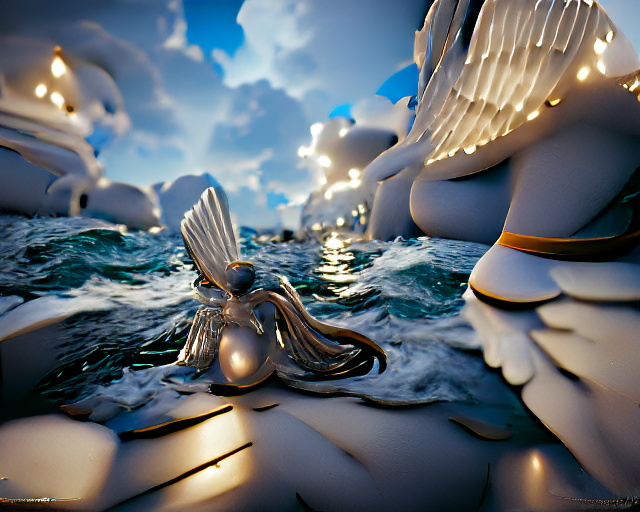
\includegraphics[width=0.8\textwidth]{img/vqgan_image.png}
    \caption{Arte generado por redes generativas adversas complementadas con \textit{transformers}}
    \label{fig:vqgan_image}
\end{figure}

\section{Requerimientos energéticos de las redes neuronales}
\label{sec:requerimientos_energeticos_redes_neuronales}
Estas a cada año más increíbles capacidades de las redes neuronales artificiales no vienen sin coste. El coste de personal de investigación y desarrollo, así como el coste energético del proceso de entrenamiento siguen siendo exageradamente altos para proyectos complejos como los citados en la Sección \ref{sec:ultimos_avances_tecnologias}.

Sin embargo en este trabajo no se trata el proceso de desarrollo y entrenamiento, ya que eso queda delegado en los muchos y muy competentes ingenieros en inteligencia artificial. En este trabajo se trata el proceso de inferencia, es decir, la ``ejecución'' de una red creada y entrenada.

El proceso de inferencia es mucho más sencillo y computacionalmente menos demandante que el de entrenamiento, pero tras esa falsa sensación de ``gratuidad'' de bajos recursos computacionales se oculta una trampa en la escala de dichos recursos. Esto es debido a que, a pesar de que una red neuronal durante el proceso de desarrollo se entrena múltiples veces con un elevado coste asociado, este entrenamiento es habitualmente llevado a cabo por un pequeño grupo de ingenieros. Por otro lado, si bien la ejecución de redes neuronales es mucho más barata computacionalmente hablando, la escala de estas redes neuronales, especialmente de las que aspiran a convertirse en parte de nuestras vidas, hace que un consumo de unos pocos mWh se convierta en varios kWh o incluso MWh por dispositivo a lo largo de todo el planeta.

Añadiendo a esto que se pretende que en el futuro prácticamente cualquier bien de consumo tenga inteligencia artificial asociada, la demanda de energía pasa a ser una preocupación importante, en la escala de los TWh. Es debido a esto que una reducción del 10\% del consumo, a pesar de parecer un logro menor, es muy importante para la sostenibilidad a largo plazo de nuestro planeta y estilo de vida.

\section{Investigación y optimizaciones propuestas}
\label{sec:investigacion_optimizaciones_propuestas}
AUUUAUAUAUAU